% -*- latex -*-
%%%%%%%%%%%%%%%%%%%%%%%%%%%%%%%%%%%%%%%%%%%%%%%%%%%%%%%%%%%%%%%%
%%%%%%%%%%%%%%%%%%%%%%%%%%%%%%%%%%%%%%%%%%%%%%%%%%%%%%%%%%%%%%%%
%%%%
%%%% This text file is part of the source of 
%%%% `Parallel Programming in MPI and OpenMP'
%%%% by Victor Eijkhout, copyright 2012-8
%%%%
%%%%
%%%%%%%%%%%%%%%%%%%%%%%%%%%%%%%%%%%%%%%%%%%%%%%%%%%%%%%%%%%%%%%%
%%%%%%%%%%%%%%%%%%%%%%%%%%%%%%%%%%%%%%%%%%%%%%%%%%%%%%%%%%%%%%%%

\Level 0 {Distributed computing and distributed data}

One reason for using MPI is that sometimes you need to work on
more data than can fit in the memory of a single processor.
With distributed memory, each processor then gets a part
of the whole data structure and only works on that.

So let's say we have a large number array, and we want to
distribute the data over the processors.
That means that, with \n{p} processes and \n{n}~elements
per processor, we have a total of $\n{n}\cdot\n{p}$ elements.

\begin{figure}[ht]
  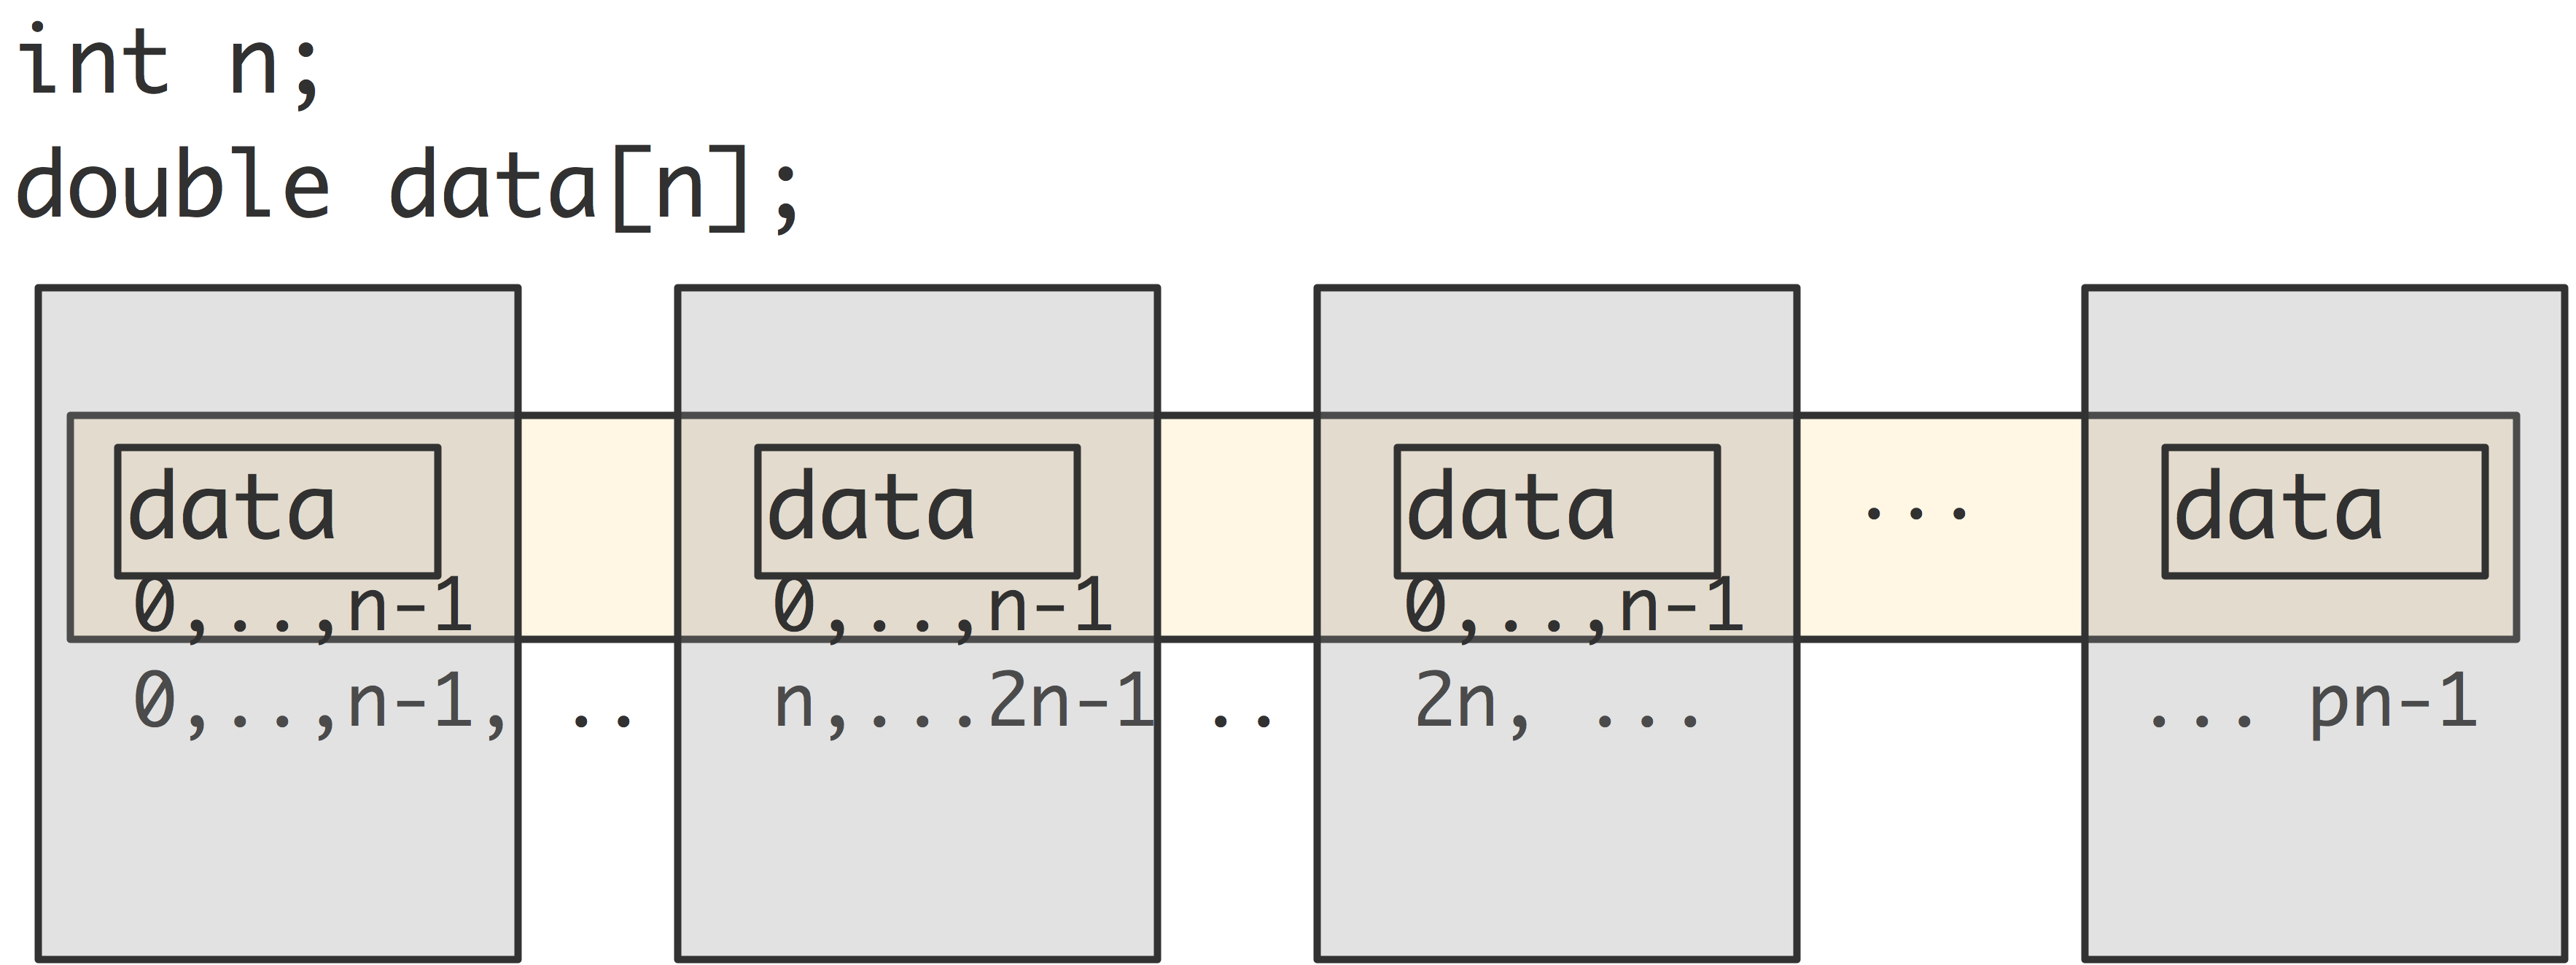
\includegraphics[scale=.1]{mpi-array}
  \caption{Local parts of a distributed array}
  \label{fig:mpi-array}
\end{figure}

We sometimes say that \n{data} is the local part
of a \indexterm{distributed array} with a total size of
$\n{n}\cdot\n{p}$ elements.
However, this array only exists
conceptually: you have to write your code in such a way that
it acts like you're working with a large distributed array.

\begin{exercise}
  We want to compute $\sum_{n=1}^Nn^2$, and we do that as follows.
  Read in the \n{Nglobal} parameter, and assume that it is a multiple
  of the number $P$ of processors. (Your code should produce an error message and
  exit immediately if it doesn't.)

  \begin{itemize}
  \item Now allocate the local parts: each processor should allocate only $N/P$ elements.
  \item Initialize your array so that the $i$-th location of the distributed array
    (for $i=0,\ldots,N-1$)
    contains~$(i+\nobreak 1)^2$.
  \item Now use a collective operation to compute the sum of the array values.
    The right value is $(2N^3+3N^2+N)/6$. Is that what you get?
  \end{itemize}
\end{exercise}

If the array size is not perfectly divisible by the number of processors,
we have to come up with a division that is uneven, but not too much.
You could for instance, write
\begin{lstlisting}
int Nglobal, // is something large
    Nlocal = Nglobal/ntids,
    excess = Nglobal%ntids;
if (mytid==ntids-1) 
  Nlocal += excess;
\end{lstlisting}

\begin{exercise}
  Read the section \HPSCref{sec:load} about load balancing, and argue that this strategy
  is not optimal. Can you come up with a better distribution?
\end{exercise}

\Level 0 {Local information exchange}

Suppose you have an array of numbers $x_i\colon i=0,\ldots,N$
and you want to compute $y_i=(x_{i-1}+x_i+x_{i+1})/3\colon i=1,\ldots,N-1$.
As before (see figure~\ref{fig:mpi-array}), we give each processor
a subset of the~$x_i$s and $y_i$s.
Let's define $i_p$ as the first index of~$y$ that is
computed by processor~$p$. (What is the last index computed by processor~$p$?
How many indices are computed on that processor?)

We often talk about the \indexterm{owner computes}
model of parallel computing: each processor `owns' certain data items,
and it computes their value.

Now let's investigate how processor~$p$ goes about computing~$y_i$ for
the $i$-values it owns. Let's assume that processor~$p$ also stores
the values $x_i$ for these same indices.
Now, it can compute
\[ y_{i_p+1} = (x_{i_p}+x_{i_p+1}+x_{i_p+2})/3 \]
and likewise $y_{i_p+2}$ and so on. However, there is a problem with
\[ y_{i_p} = (x_{i_p-1}+x_{i_p}+x_{i_p+1})/3 \]
since $x_{i_p}$ is not stored on processor~$p$: it is stored on~$p-\nobreak1$.

There is a similar story with the last index that $p$ tries to compute:
that involves a value that is only present on~$p+1$.

You see that there is a need for processor-to-processor, or technically \indexterm{point-to-point},
information exchange.

\Level 1 {Ping-pong}

A simple scenario for information exchange between just two processes is the \indexterm{ping-pong}:
process~A sends data to process~B, which sends data back to~A.

Read section~\ref{sec:mpi-timing}, and in particular~\ref{sec:ping-time}. Do the exercises.

\Level 1 {Pairwise exchange}

\begin{exercise}
  Implement the above averaging scheme using \indexmpishow{MPI_Sendrecv}.
\end{exercise}

\begin{exercise}
  Do exercise~\ref{ex:exchange-sort}
\end{exercise}

\begin{exercise}
  Implement the above averaging scheme using \indexmpishow{MPI_Isend} and \indexmpishow{MPI_Irecv}.
\end{exercise}

\Level 1 {Neighbourhood exchange}

\indexmpishow{MPI_Dist_graph_create}

